\documentclass[tikz]{standalone}
\usetikzlibrary{shapes,arrows.meta}
\begin{document}
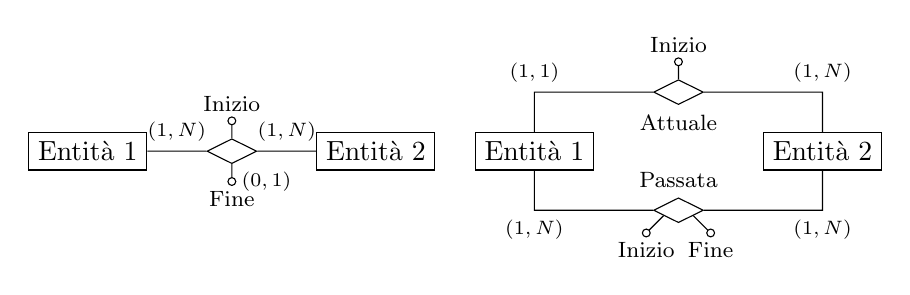
\begin{tikzpicture}
    \draw

    %%* Attributi:
    %%  node[draw, circle, inner sep=1pt,anchor=180, fill=black]{}node[right]{\footnotesize A}
    %%? Distanza orizzontale: E -(0.25,0.x)- A
    %%? Distanza verticale: E -(0,x * 0.22)- A

    %%* Cardinalità:
    %%  node[below right]{\scriptsize $(0,N)$}
    %%  node[above right]{\scriptsize $(0,N)$}
    %%  node[midway, above]{\scriptsize $(0,N)$}

    %%* Relazione:
    %%  node[draw, diamond, shape aspect=2, inner sep=3pt, anchor=90](r1){}
    %%  node[draw, diamond, shape aspect=2, inner sep=0.2pt, anchor=180](r2){R2}

    %%* Entità:
    %%  node[draw, rectangle, anchor=90](e1){}
    %%? Distanza verticale: E -(0.3)- R -(0.3) E
    %%? Distanza orizzontale: E -(0.75)- R -(0.75)- E

    %%* Entità 1
    (0,0)node[draw, rectangle, anchor=180](e1){Entità 1}


    %%* Relazione
    (e1.0)--++(0.75,0)node[midway, above]{\scriptsize $(1,N)$}node[draw, diamond, shape aspect=2, inner sep=3pt, anchor=180](r1){}

    (r1.90)--++(0,0.22)node[draw, circle, inner sep=1pt, fill=white]{}node[above]{\footnotesize Inizio}
    (r1.270)--++(0,-0.22)node[draw, circle, inner sep=1pt, fill=white]{}node[below]{\footnotesize Fine}node[right]{\scriptsize $(0,1)$}
    
    %%* Entità 2
    (r1.0)--++(0.75,0)node[midway, above]{\scriptsize $(1,N)$}node[draw, rectangle, anchor=180](e2){Entità 2}


    %%* Entità 1
    (e2.0)++(0.5,0)node[draw, rectangle, anchor=180](e1){Entità 1}

    %%* Relazioni
    (e1.0)++(0.75,0.75)node[draw, diamond, shape aspect=2, inner sep=3pt, anchor=180, label=below:{\footnotesize Attuale}](r1){}
    (r1.90)--++(0,0.22)node[draw, circle, inner sep=1pt, fill=white]{}node[above]{\footnotesize Inizio}
    
    (e1.0)++(0.75,-0.75)node[draw, diamond, shape aspect=2, inner sep=3pt, anchor=180, label=above:{\footnotesize Passata}](r2){}
    
    (r2.200)--++(-0.22,-0.22)node[draw, circle, inner sep=1pt, fill=white]{}node[below]{\footnotesize Inizio}
    (r2.340)--++(0.22,-0.22)node[draw, circle, inner sep=1pt, fill=white]{}node[below]{\footnotesize Fine}

    %%* Entità 2
    (r1.0)++(0.75,-0.75)node[draw, rectangle, anchor=180](e2){Entità 2}

    (e1.90)|-(r1.180)node[midway, above]{\scriptsize $(1,1)$}
    (r1.0)-|(e2.90)node[midway, above]{\scriptsize $(1,N)$}
    (e1.270)|-(r2.180)node[midway, below]{\scriptsize $(1,N)$}
    (r2.0)-|(e2.270)node[midway, below]{\scriptsize $(1,N)$}

    ;
\end{tikzpicture}
\end{document}